
The notion of access control (AC) and application/process isolation is one of the oldest in the history of information security with first pioneering works done back in the 70s~\cite{saltzer75, Denning76}. Initially the main goal of AC methods was to isolate different system's users with different level of access to the system assets, but as the computers and other IT devices started to become more and more single-user purpose, the focus has shifted towards isolation of system processes and applications\footnote{in case a process or application becomes compromised, one wants to have the rest of the system and user's data protected}.
 This trend was especially noticeable in various mobile platform security architectures, when the users got the ability to install third-party software on their mobile devices: it required a stricter isolation between system's core platform and services (trusted set of entities) and user installable services and applications (untrusted and potentially malicious).

A typical AC system can be viewed as a collection of one or more AC reference monitors that are consulted for AC decisions whenever any system access (such as operation on a filesystem object) is performed. The AC decision is done based on the AC policy for that AC reference monitor and defines if the access should be allowed or not. The AC policy is written in a form of AC rules that are defined in terms of \textit{subjects} (active entity performing the access), \textit{objects} (passive entity that is being accessed) and \textit{access types} (type of access being attempted, such as read, write etc.). Subject and objects are also typically grouped into a set of \textit{access control domains} using some identification or labeling scheme, allowing policy writers to arrange related and interconnected OS components into logical blocks. Typically most of the AC systems employ the principle that by default any access is denied unless explicitly allowed by AC policy rules, or both subject and object are belonging to the same access control domain.
 
Over the decades the topic of process and application isolation was a focus of tremendous amount of academia and industrial research works: many systems and mechanisms were proposed to address the problems arising when designing and implementing AC systems. On a high level these problems can be arranged into the following categories that are all interconnected and affect each other: 

\begin{itemize}
	\item \textbf{Granularity.} One can design and deploy AC mechanisms with very different granularity levels following the principle of least privilege. On one side one can place each individual process or even process thread into its own access control domain, and on the other side only create high-level access control domains that would isolate the trusted part of the system from user-installable and less trusted applications. It is clear that a fine-grained AC policy allows creating a more precise set of AC rules for a given AC object. However it usually directly negatively impacts other factors like manageability and performance, forcing AC policy's creators to search for some intermediate balance.
	\item \textbf{Manageability.} Most modern mobile and embedded OSes change at a high pace: new system services and APIs being introduced with each release, existing services might be fully redesigned, new use cases might be introduced etc. Same applies for the systems AC policy: it must adapt and change with the OS to make sure it not only correctly reflects the current state of the system, but also correctly isolates and protects its entities. In addition, one needs to take into account how OS is being developed. For example if OS changes are done in distributed fashion by different independent set of development teams, the policy needs to be modular enough to allow changes to be performed relatively independently and in parallel. One just cannot assume that there is a single person that can manage all policy changes centrally.  
	\item \textbf{Performance.} Typically an access control system is integral part of an OS and for every system access, an access control decision needs to be made based on available parameters. This makes an AC mechanism a very run-time performance sensitive component and care needs to be taken to make the overhead acceptable for system use. 
\end{itemize}

Part of this thesis investigates how the modern AC mechanisms attempt to find a balance in the above categories, what are the concrete problems that they are facing in the struggle to find this balance, as well as to understand what tools or techniques can be helpful in practice to solve these problems. For this purpose the thesis selects one of the most popular mobile operating system, Android, and its mandatory AC mechanism, SEAndroid~\cite{smalley12}, for a detailed evaluation as the most used mandatory AC mechanism on mobile Linux-based OSes. Another focus area of this thesis is an attempt to look into alternative ways how process and application isolation can be done using various OS-level virtualization  techniques that during the last couple of years became a fashionable alternative to traditional AC mechanisms. The main research question that this thesis attempts to answer with regards to the OS-level virtualization is whether this technique can provide a similar level of security as traditional mandatory AC mechanisms. 


\section{Mandatory access control on modern systems: SEAndroid}

Over the past decades, Android has become one of the most common OSes for mobile devices. As the amount of devices running Android has been increasing, so has the amount of malware targeting this operating system. Back in 2011 it became clear that the discretionary Android permission access control model is not able to provide the required level of security and the work started on adapting the well-known desktop mandatory access control mechanism, SELinux, for the purpose of Android OS. The resulting mechanism, SEAndroid~\cite{smalley12}, was largely based on SELinux, but contained some adjustments and additions required for supporting some of Android-specific mechanisms, such as Binder Inter Process Communication (IPC)~\cite{binder}. The biggest change was the SEAndroid reference policy, which was written from scratch due to significant differences between the Android and typical Linux desktop userspace layers, as well as a desire to have a small and compact policy. The initial policy and enforcement points were added to the Android 4.3 release back in 2012, but it wasn't until Android 5.0 Lollipop release when SEAndroid was requested to be enabled on all devices in the system-wide enforcing mode, which forced OEMs to start working on their SEAndroid policies. 

Traditionally the Android ecosystem works in a way that Google delivers the reference code for the Android OS in a form of open source AOSP project~\cite{aosp}. Next this code is taken by different Android OEMs and customized at various levels including HW adaption, new OEM-specific drivers and system services, new user facing applications. The reference SEAndroid policy, provided by the AOSP project, does not obviously cover these additions and customizations, and therefore OEMs need to adjust the provided SEAndroid policy, not only to get to a desired level of mandatory access control enforcement, but also merely to make their customized Android OS function correctly.

Publication II of this thesis starts by examining 8 different SEAndroid policies (taken from the Android 5.0 release) from various Android OEMs and provides extensive characteristics of these policies in terms of OEM-performed changes, policy size, complexity and etc. Table 1 from Publication II shows that all OEMs extensively modify the reference policy resulting in overall policy size growth, as well as all other policy attributes and access control rules. Next Publication II manually analyzes the characteristics of each of these 8 policies and builds a set of typical pitfalls that all OEMs make when performing their policy additions. These include \textit{overuse of default types}, where many OEMs leave SEAndroid default labels\footnote{if an object is not given an explicit label by the SEAndroid policy, it is assigned one of the default labels, such as \setype{unlabeled}, \setype{device}, \setype{default\_prop} etc.} for their newly added system objects. This typically leads to aggregation of big amount of non-related objects under a single default label and consequently violates the principle of least privilege: many different processes end up having a legitimate access to the objects under default labels. Another typical pitfall is the \textit{aggregation of OEM-created applications under few AOSP-predefined application domains}, such as \setype{platform\_app} or \setype{system\_app} instead of defining smaller, OEM-specific application domains. This leads to the enormous grow of such default domains (for example one OEM policy had 900 allow rules associated with \setype{system\_app} domain vs. 46 in the AOSP reference policy) and inability to prevent privilege escalation between different OEM applications placed in these domains. Other OEMs pitfalls include \textit{seemingly useless or forgotten rules} present in their policies, as well as \textit{rules that are dangerous for the overall security of the system} (such as granting access to rather sensitive parts of the system to untrusted domains). All of these pitfalls indicate that for the Android 5.0 release OEMs struggled to deliver the comprehensive and secure SEAndroid policies on their devices. 

\begin{figure}[t]
	\centering
		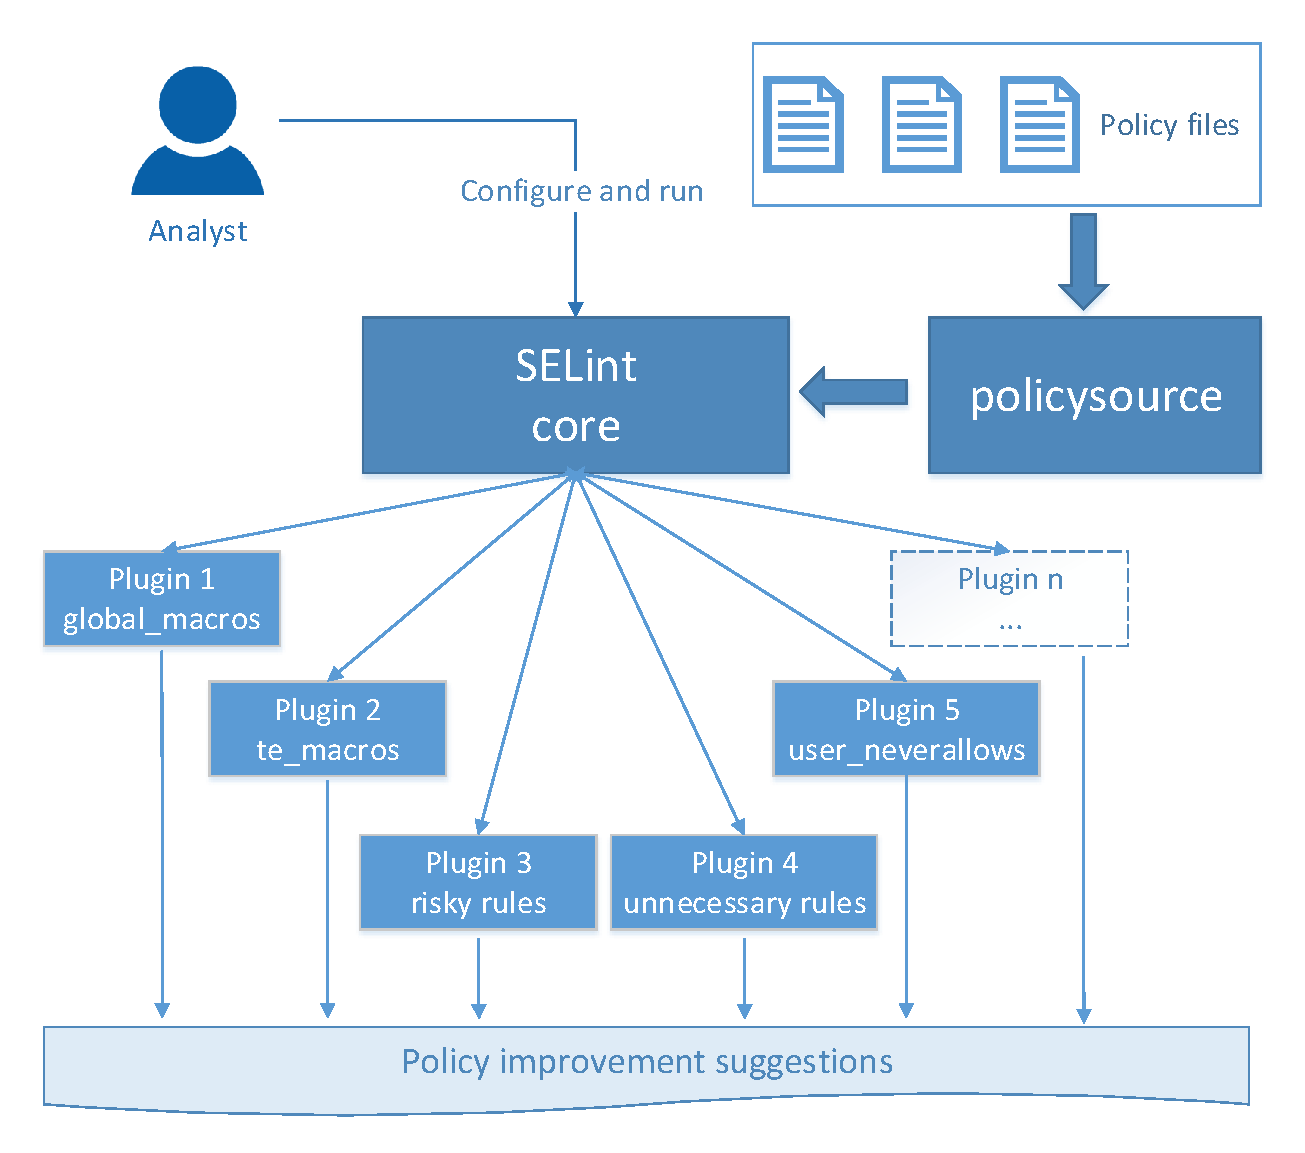
\includegraphics[width=0.80\textwidth]{figures/selint-archi.pdf}
	\caption{The architecture of SELint (Adapted from Publication III)}
	\label{fig:selint}
\end{figure}

As a result of above study, Publication II proposes a set of tools that should help both OEMs and security researchers to develop better SEAndroid policies without the above-mentioned pitfalls, including various policy analyzers and virtualization tools. It also implements one such tool, a live SEAndroid policy analyzer (SEAL), that allows performing different policy queries, not only based on the actual policy loaded on a device, but also also based on the run-time device state, i.e. running processes and services, filesystem labeling etc. SEAL allows obtaining fast answers on various questions that a SEAndroid policy writer or analyzer might have, such as "\textit{What files can a given running process access on a device?}" or "\textit{What processes can access a given object?}". This significantly simplifies the debugging, troubleshooting and studying the given SEAndroid policy and gives a fast way to discover the inconsistencies. 

Publication III presents the design and implementation of a more comprehensive SEAndroid tool, SELint, that aims to improve the SEAndroid policy development. It operates on the SEAndroid policy sources and allows smooth integration into the OEM policy development workflow. The architecture of SELint is shown in Figure~\ref{fig:selint}. It is composed from a SELint core, responsible for the heavy processing of input SEAndroid policy files, and an initial set of SELint plugins that operate on a policy representation provided by the core and able to do the policy analysis. The set of plugins is designed to be extensible and adapt to the needs of different OEMs or security researchers. The initial set of plugins includes five distinct ones: two plugins (\setype{global\_macros} and \setype{te\_macros}) verifying correctness of usage different types of SEAndroid policy macros, a \setype{user\_neverallows} plugin that allows a OEM-specific verification of additional neverallow rules, a \setype{unnecessary\_rules} plugin that attempts to detect various ineffective rules\footnote{some rules in SEAndroid policy are only effective in combination with others, such as domain transition rules when a process wants to transition its domain to a different one upon opening a certain type of object} or rules used for debug purposes, and finally a \setype{risky\_rules} plugin that can be used to categorize SEAndroid access control domains into set of related ones (untrusted, security-sensitive, core etc.) and display various risk and trust relationships between them in a given policy. For example, it is possible to highlight the access control rules where the access to a security-sensitive object is given to a subject belonging to an untrusted domain.


\section{Application and process isolation using OS-level virtualization}
\label{sec:os-virt}

While traditional access control mechanisms and systems aiming for application and process isolation have existed for decades, recent years have seen a raise of an alternative approach, \textit{OS-level virtualization techniques}, widely known as "\textit{containers}". While originally developed purely to support various virtualization-based use cases, such as server consolidation or application and resource state management, they later on turned into various security-driven use cases, such as application isolation and the Bring Your Own Device (BYOD) scenario\footnote{a single physical device is used for both business and personal purposes that requires a strict isolation between these two environments and limited sharing}. These additional focus areas brought new security requirements towards application and process isolation for OS-level virtualization techniques.

In contrary to the traditional virtualization solutions, like well-known Xen hypervisor~\cite{xenproject} or Linux Kernel Virtual Machine (KVM)~\cite{kvmproject}, an OS-level virtualization only virtualizes the OS kernel resources available to userspace, as opposed to the actual physical HW resources, and therefore allows processes to share the same host OS kernel. This greatly reduces the performance overhead incurred by the OS-level virtualization and consequently becomes possible to use this technology for an efficient isolation of stand-alone applications or their sets. Parallel to their popularity, there is a constant debate about the security level that such virtualization provides in practice, as well as an attempt to find the gaps in the current implementation. 


\begin{figure}[t]
\centering
\begin{subfigure}{.5\textwidth}
  \centering
  \includegraphics[width=0.8\linewidth]{figures/os-virtualization-sys-model.png}
  \caption{System model}
  \label{fig:osv-1}
\end{subfigure}%
\begin{subfigure}{.5\textwidth}
  \centering
  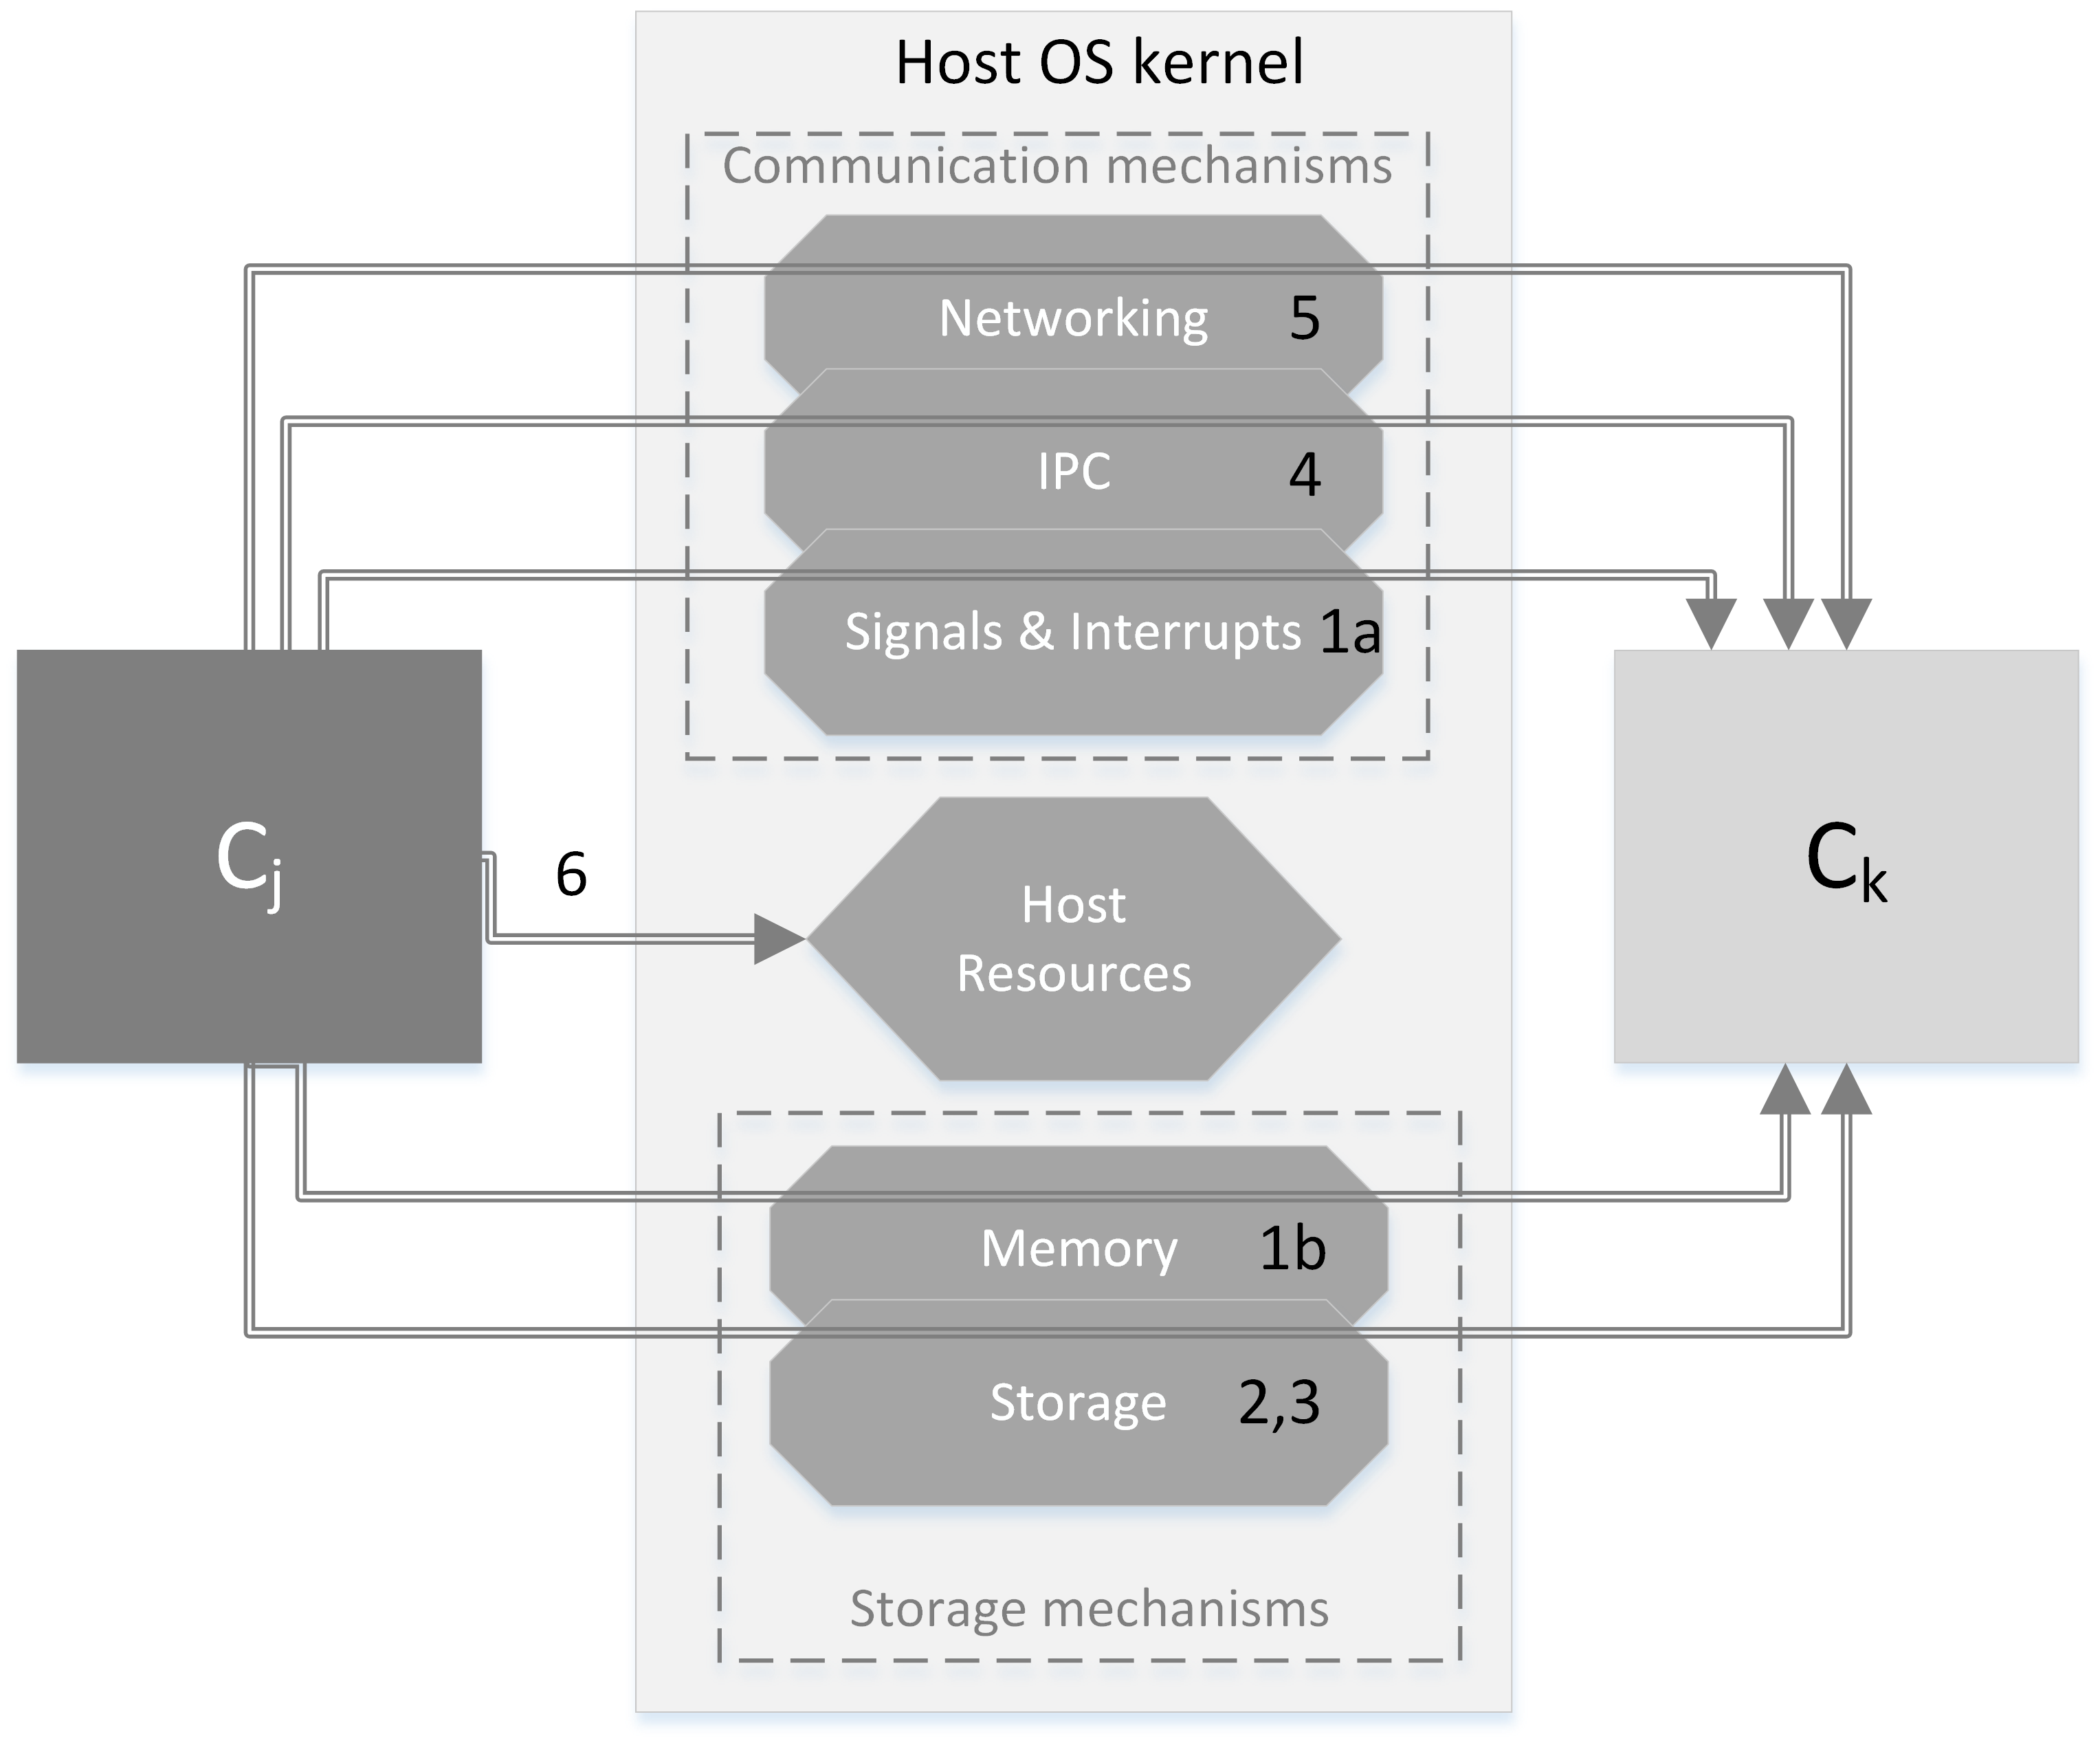
\includegraphics[width=1\linewidth]{figures/OS-virtualization-attacker-model.png}
  \caption{Attacker model}
  \label{fig:osv-2}
\end{subfigure}
\caption{OS-level virtualization. (Adapted from Publication VI)}
\label{fig:os-virtualization}
\end{figure}

Publication IV of this thesis identifies the security requirements and generic model for a typical OS-level virtualization setup.
The system model for OS-level virtualization is shown in Figure~\ref{fig:osv-1}. The set of containers \setype{C\scriptsize{1}\normalsize..C\scriptsize{N}} is running on top of a shared host OS kernel and a userspace layer. The latter one can be either a minimal layer, only responsible for doing the setup of containers, or a full-fledged host OS userspace layer. The attacker model shown in Figure~\ref{fig:osv-2} assumes that an adversary has full control over a certain subset of containers and attempts to attack either another subset of legitimate containers running on the same host or the host OS itself. An attacker aims to achieve one of the following end goals: privilege escalation, legitimate container or host compromise or denial-of-service. This can be done by one of the attack groups 1 to 6 shown in Figure~\ref{fig:osv-2}, classified based on typical interfaces available to a UNIX-compliant OS. These attack groups are then converted into security requirements that each OS-level virtualization solution must fulfill in order to provide strong isolation guarantees: separation of processes, filesystem isolation, device isolation, IPC isolation, network isolation and resource management.   

Publication IV analyzes 6 different OS-level virtualization solutions against the above security requirements and outlines the differences in the provided level of isolation. It also summaries the state of OS-level virtualization in the mainline Linux kernel, implemented using "\textit{kernel namespaces}"~\cite{biederman2006}. A \textit{kernel namespace} is a set of identifiers representing the global kernel resources, such as process and user ids, filesystem mounts, network interfaces, IPC objects, etc. A \textit{container} in the mainline Linux kernel is therefore a collection of such kernel namespaces that restrict visibility and communication between processes running in different kernel namespaces. In addition, Publication IV also defines a number of gaps that were limiting the usage of this technology in the environments with strict security isolation requirements: the need for security namespaces, a better support for resource management, etc. In recent years some of these gaps have progressed towards a robust solution and many new ones have been identified. Below is the summary of changes in the relevant areas that help improving the OS-level virtualization in the mainline Linux kernel:  

\begin{itemize}
	\item \textbf{Security (LSM) namespaces.} Publication IV outlines the importance of having security namespaces implemented in order to be able to enforce independent mandatory access control security policies for different containers, as well as for the host OS. In recent years this topic has been of a great focus for the Linux kernel security community with a number of mainstream Linux Security Modules (LSMs), such as Smack~\cite{smack} and AppArmor~\cite{bauer2006paranoid}, proposing their approaches and implementations~\cite{smackns},~\cite{apparmorns}. Unfortunately these implementations are currently LSM-specific and only allow creation of independent container-specific policies within the same LSM. However, this is a significant step forward and discussions on a unified solution continue.
	\item \textbf{Cgroups support.} \setype{cgroups} kernel subsystem~\cite{cgroupsv2}, that is actively used in the mainline Linux kernel to implement resource management, has undergone a major change at the end of 2015 in an attempt to address various gaps and criticism from its users~\cite{rosen2016}. The new solution, \setype{cgroups v2}~\cite{cgroupsv2}, added many new features, including an ability to apply controls per thread granularity (which used to be possible with an old \setype{rlimits} technology) as well as namespace support for \setype{cgroups} themselves. Latter allows having independent \setype{cgroup} hierarchies for different containers and restricts each container to only view its own \setype{cgroups} rules. 
	\item \textbf{Automatic loading restriction support.} A process running inside a malicious container might try to use kernel features like automatic module loading as a way to escape the container. It can be done by requesting a kernel feature that is provided by a module that is not loaded in the kernel. In order to satisfy the request, the kernel would automatically load the module, despite the process having no permissions to ask about such operation explicitly. In turn this module can be potentially an old and vulnerable one exposing the host OS kernel for easy attacks. A recent proposal~\cite{harouni2017} to address this issue and create suitable controls has been discussed in the mainline Linux kernel community, and while the implementation details will still likely change, it is considered as an important security improvement. 
  \item \textbf{Keyring namespace support.} The mainline Linux kernel has a convenient facility, \textit{Kernel Keyring}~\cite{keyrings}, for in-kernel storage and manage of security keys and authentication tokens. The keys stored in these \textit{keyrings} are available not only for usage within the kernel itself, but also for userspace processes. From security point of view, different containers and host OS should naturally have separated kernel keyrings, but this hasn't yet been implemented in the mainline Linux kernel. Similar to other cases, an initial proposal~\cite{howells2016} by the keyring subsystem maintainer that separates keyrings between different user namespaces has been discussed by the Linux kernel security community and remains the expected future direction. 
	\item \textbf{IMA policy namespaces.} In addition to MAC mechanisms provided by various LSMs, the mainline Linux kernel has an Integrity Measurement Architecture (IMA)~\cite{ima} subsystem that aims to detect if files have been accidentally or maliciously modified when device is in the offline state. This is done by calculating a reference hash value over the file content and attributes and comparing it to newly calculated value every time the file is accessed. Similarly as for LSMs, IMA operates on a policy that defines what files should be measured and when, as well as various exceptions. OS-level virtualization brings a similar requirement to IMA as for LSMs: the IMA policy needs to be namespaced in order to be able to have separate independent policies for host OS and different containers. Active discussions on the best direction for IMA policy namespacing continues in the Linux kernel security community as well as first implementation proposals have been presented~\cite{magalhaes2017}. 
	\item \textbf{Stricter handling of POSIX capabilities.} A very recent proposal~\cite{Bandewar2017} introduces a mechanism to limit the usage of POSIX capabilities~\cite{caps} inside user namespaces. This can be a very desired feature for further security hardening for OS-level virtualization since it is currently possible for a process that entered a user namespace to acquire a wide range of POSIX capabilities within this namespace and try to misuse them. 
\end{itemize}


\section{Discussion}

OS-level virtualization methods gained a lot of attention and interest in the Linux community due to their usability aspects. It is much easier to spawn a set of separate containers with independently running applications than achieving the same setup using MAC mechanisms. However, if sharing of data or IPC communication between these applications is required, then the setup quickly gets more complicated. Additionally while the implementation of the OS-level virtualization in the mainline Linux kernel continues to evolve and improve, the classical mandatory access control schemes are still required to be jointly used in order to provide the highest possible level of isolation and minimize the security risks. Security architects must understand the details and the limitations of OS-level virtualization in order to make well-grounded choices on a set of isolation mechanisms for their systems in order to fulfill given security requirements. Publication IV of this thesis presents a good model for such evaluation and comparison of available mechanisms, as well as guidance on identifying the missing isolation gaps. 

The SEAndroid MAC continues to be the main AC enforcement point of Android OS with all major OEMs now accustomed to the task of working with SEAndroid policies. The evaluation of initial SEAndroid policies done in Publication II has been crossed-referenced in the official Google SEAndroid documentation as a valuable insight into practical state of things~\cite{seanroidsize}. The SEAndroid tools, proposed in Publications II and III, are being used by the Android community with numerous private forks done on the project code trees and bug reports filled by the users once in a while\footnote{https://github.com/seandroid-analytics}. The SELint tool fulfills the set of its main functional R1 - R4 requirements defined in Section IV of Publication III by exhibiting an acceptable performance overhead, allowing its usage by ordinary users (after an initial expert configuration), being flexible and easy extensible. Due to the nature of SELint, i.e. the tool is targeting OEMs and internal use within their systems, it is hard to make an estimate on its usage in the real world, but a detailed evaluation of the tool can be found in Section V of Publication III. 

